\documentclass[]{article}
\usepackage{lmodern}
\usepackage{amssymb,amsmath}
\usepackage{ifxetex,ifluatex}
\usepackage{fixltx2e} % provides \textsubscript
\ifnum 0\ifxetex 1\fi\ifluatex 1\fi=0 % if pdftex
  \usepackage[T1]{fontenc}
  \usepackage[utf8]{inputenc}
\else % if luatex or xelatex
  \ifxetex
    \usepackage{mathspec}
    \usepackage{xltxtra,xunicode}
  \else
    \usepackage{fontspec}
  \fi
  \defaultfontfeatures{Mapping=tex-text,Scale=MatchLowercase}
  \newcommand{\euro}{€}
\fi
% use upquote if available, for straight quotes in verbatim environments
\IfFileExists{upquote.sty}{\usepackage{upquote}}{}
% use microtype if available
\IfFileExists{microtype.sty}{%
\usepackage{microtype}
\UseMicrotypeSet[protrusion]{basicmath} % disable protrusion for tt fonts
}{}
\usepackage[margin=1in]{geometry}
\ifxetex
  \usepackage[setpagesize=false, % page size defined by xetex
              unicode=false, % unicode breaks when used with xetex
              xetex]{hyperref}
\else
  \usepackage[unicode=true]{hyperref}
\fi
\hypersetup{breaklinks=true,
            bookmarks=true,
            pdfauthor={Instituto Tecnológico Autónomo de México; Gilberto Iglesias; Andrea Fernández Conde; Lizbeth Contreras; Amanda Barrera},
            pdftitle={Proyecto 3: Orquestación},
            colorlinks=true,
            citecolor=blue,
            urlcolor=blue,
            linkcolor=magenta,
            pdfborder={0 0 0}}
\urlstyle{same}  % don't use monospace font for urls
\setlength{\parindent}{0pt}
\setlength{\parskip}{6pt plus 2pt minus 1pt}
\setlength{\emergencystretch}{3em}  % prevent overfull lines
\setcounter{secnumdepth}{5}

%%% Use protect on footnotes to avoid problems with footnotes in titles
\let\rmarkdownfootnote\footnote%
\def\footnote{\protect\rmarkdownfootnote}

%%% Change title format to be more compact
\usepackage{titling}
\setlength{\droptitle}{-2em}
  \title{Proyecto 3: Orquestación}
  \pretitle{\vspace{\droptitle}\centering\huge}
  \posttitle{\par}
  \author{Instituto Tecnológico Autónomo de México \\ Gilberto Iglesias \\ Andrea Fernández Conde \\ Lizbeth Contreras \\ Amanda Barrera}
  \preauthor{\centering\large\emph}
  \postauthor{\par}
  \predate{\centering\large\emph}
  \postdate{\par}
  \date{30/05/2015}


\usepackage{float}
\usepackage{morefloats}
\usepackage[spanish]{babel}
\usepackage{graphicx}
\usepackage{tcolorbox}
\usepackage{rotating}
\usepackage{longtable}
\usepackage{colortbl}
%\usepackage{natbib}
%\newenvironment{scaleb}{ \scalebox{0.4}{} {} }
%\newenvironment{scaleb}{ \tiny{} }
% biber
\usepackage[autostyle]{csquotes}

\usepackage[
    backend=biber,
    style=authoryear-icomp,
    sortlocale=de_DE,
    natbib=true,
    url=false,
    doi=true,
    eprint=false
]{biblatex}
\addbibresource{bibliografia.bib}

\usepackage[]{hyperref}
\hypersetup{
% Turn on this if you prefer to have links colored instead of marked with squares
colorlinks = true,
linkcolor = black,
urlcolor = blue,
citecolor = black,
% pdfpagemode = UseNone
}

\renewcommand\figurename{Figura}
\renewcommand\tablename{Tabla}

\newenvironment{myexampleblock}[1]{%
    \tcolorbox[beamer,%
    noparskip,breakable,
    colback=LightGreen,colframe=DarkGreen,%
    colbacklower=LimeGreen!75!LightGreen,%
    title=#1]}%
    {\endtcolorbox}

\newenvironment{myalertblock}[1]{%
    \tcolorbox[beamer,%
    noparskip,breakable,
    colback=LightCoral,colframe=DarkRed,%
    colbacklower=Tomato!75!LightCoral,%
    title=#1]}%
    {\endtcolorbox}

\newenvironment{myblock}[1]{%
    \tcolorbox[beamer,%
    noparskip,breakable,
    colback=LightBlue,colframe=DarkBlue,%
    colbacklower=DarkBlue!75!LightBlue,%
    title=#1]}%
    {\endtcolorbox}


\begin{document}

\maketitle


{
\hypersetup{linkcolor=black}
\setcounter{tocdepth}{3}
\tableofcontents
}
\pagebreak

\section{Introducción}\label{introduccion}

Generalmente se dice que el procesamiento a gran escala debe cumplir las
tres V's: Volumen, Velocidad y Variedad. La necesidad de procesar
información a gran escala de forma muy rápida ha llevado a la creación
de una gran variedad de soluciones con diferentes características, lo
anterior ha permitido que en la actualidad se pueda disponer de diversas
herramientas para la implementación de procesos que impliquen el
análisis de grandes cantidades de datos. Cada una de las herramientas
desarrolladas hasta la actualidad cuentan con ventajas y desventajas que
deben ser analizadas dependiendo el tipo de proyecto y análisis que se
quiera desarrollar, lo anterior permitirá identificar la herramienta que
mejor se adapte a las necesidades del proyecto a desarrollar. A
continuación se describen las características de cada una de las
herramientas utilizadas en el desarrollo de nuestro proyectos y la
implementación que se realizó.

\section{Pipeline de datos}\label{pipeline-de-datos}

\subsection{Objetivo}\label{objetivo}

Implementar el flujo para la base de datos de \textbf{GDELT}:

\begin{itemize}
\itemsep1pt\parskip0pt\parsep0pt
\item
  Obtención:

  \begin{itemize}
  \itemsep1pt\parskip0pt\parsep0pt
  \item
    Crawler
  \item
    Identificar si hay nueva información
  \item
    Bajar a zip
  \item
    Guardar en disco
  \item
    Descomprimir
  \end{itemize}
\item
  Limpieza:

  \begin{itemize}
  \itemsep1pt\parskip0pt\parsep0pt
  \item
    Revisar columnas
  \item
    Quitar columnas no requeridas
  \item
    Estructurar las columnas en un orden apropiado
  \item
    Realizar proceso de normalización de datos (e.g.~fechas a UTC)
  \item
    Enviar a un archivo de texto
  \end{itemize}
\item
  Manipulación:

  \begin{itemize}
  \itemsep1pt\parskip0pt\parsep0pt
  \item
    Detectar que se escribió un archivo de texto y triggerear la subida
    al HDFS
  \item
    Realizar un proceso de analítica que actualice la información
  \item
    Tener una base de datos para shiny actualizada
  \end{itemize}
\end{itemize}

\subsection{Herramientas a utilizar}\label{herramientas-a-utilizar}

\begin{enumerate}
\def\labelenumi{\arabic{enumi}.}
\itemsep1pt\parskip0pt\parsep0pt
\item
  Sistema de carpetas / configuración / docker
\item
  Flume
\item
  Luigi
\item
  Spark
\item
  Sqoop
\item
  Hive/Impala
\end{enumerate}

\subsection{Implementación}\label{implementacion}

\begin{figure}[H]
\centering
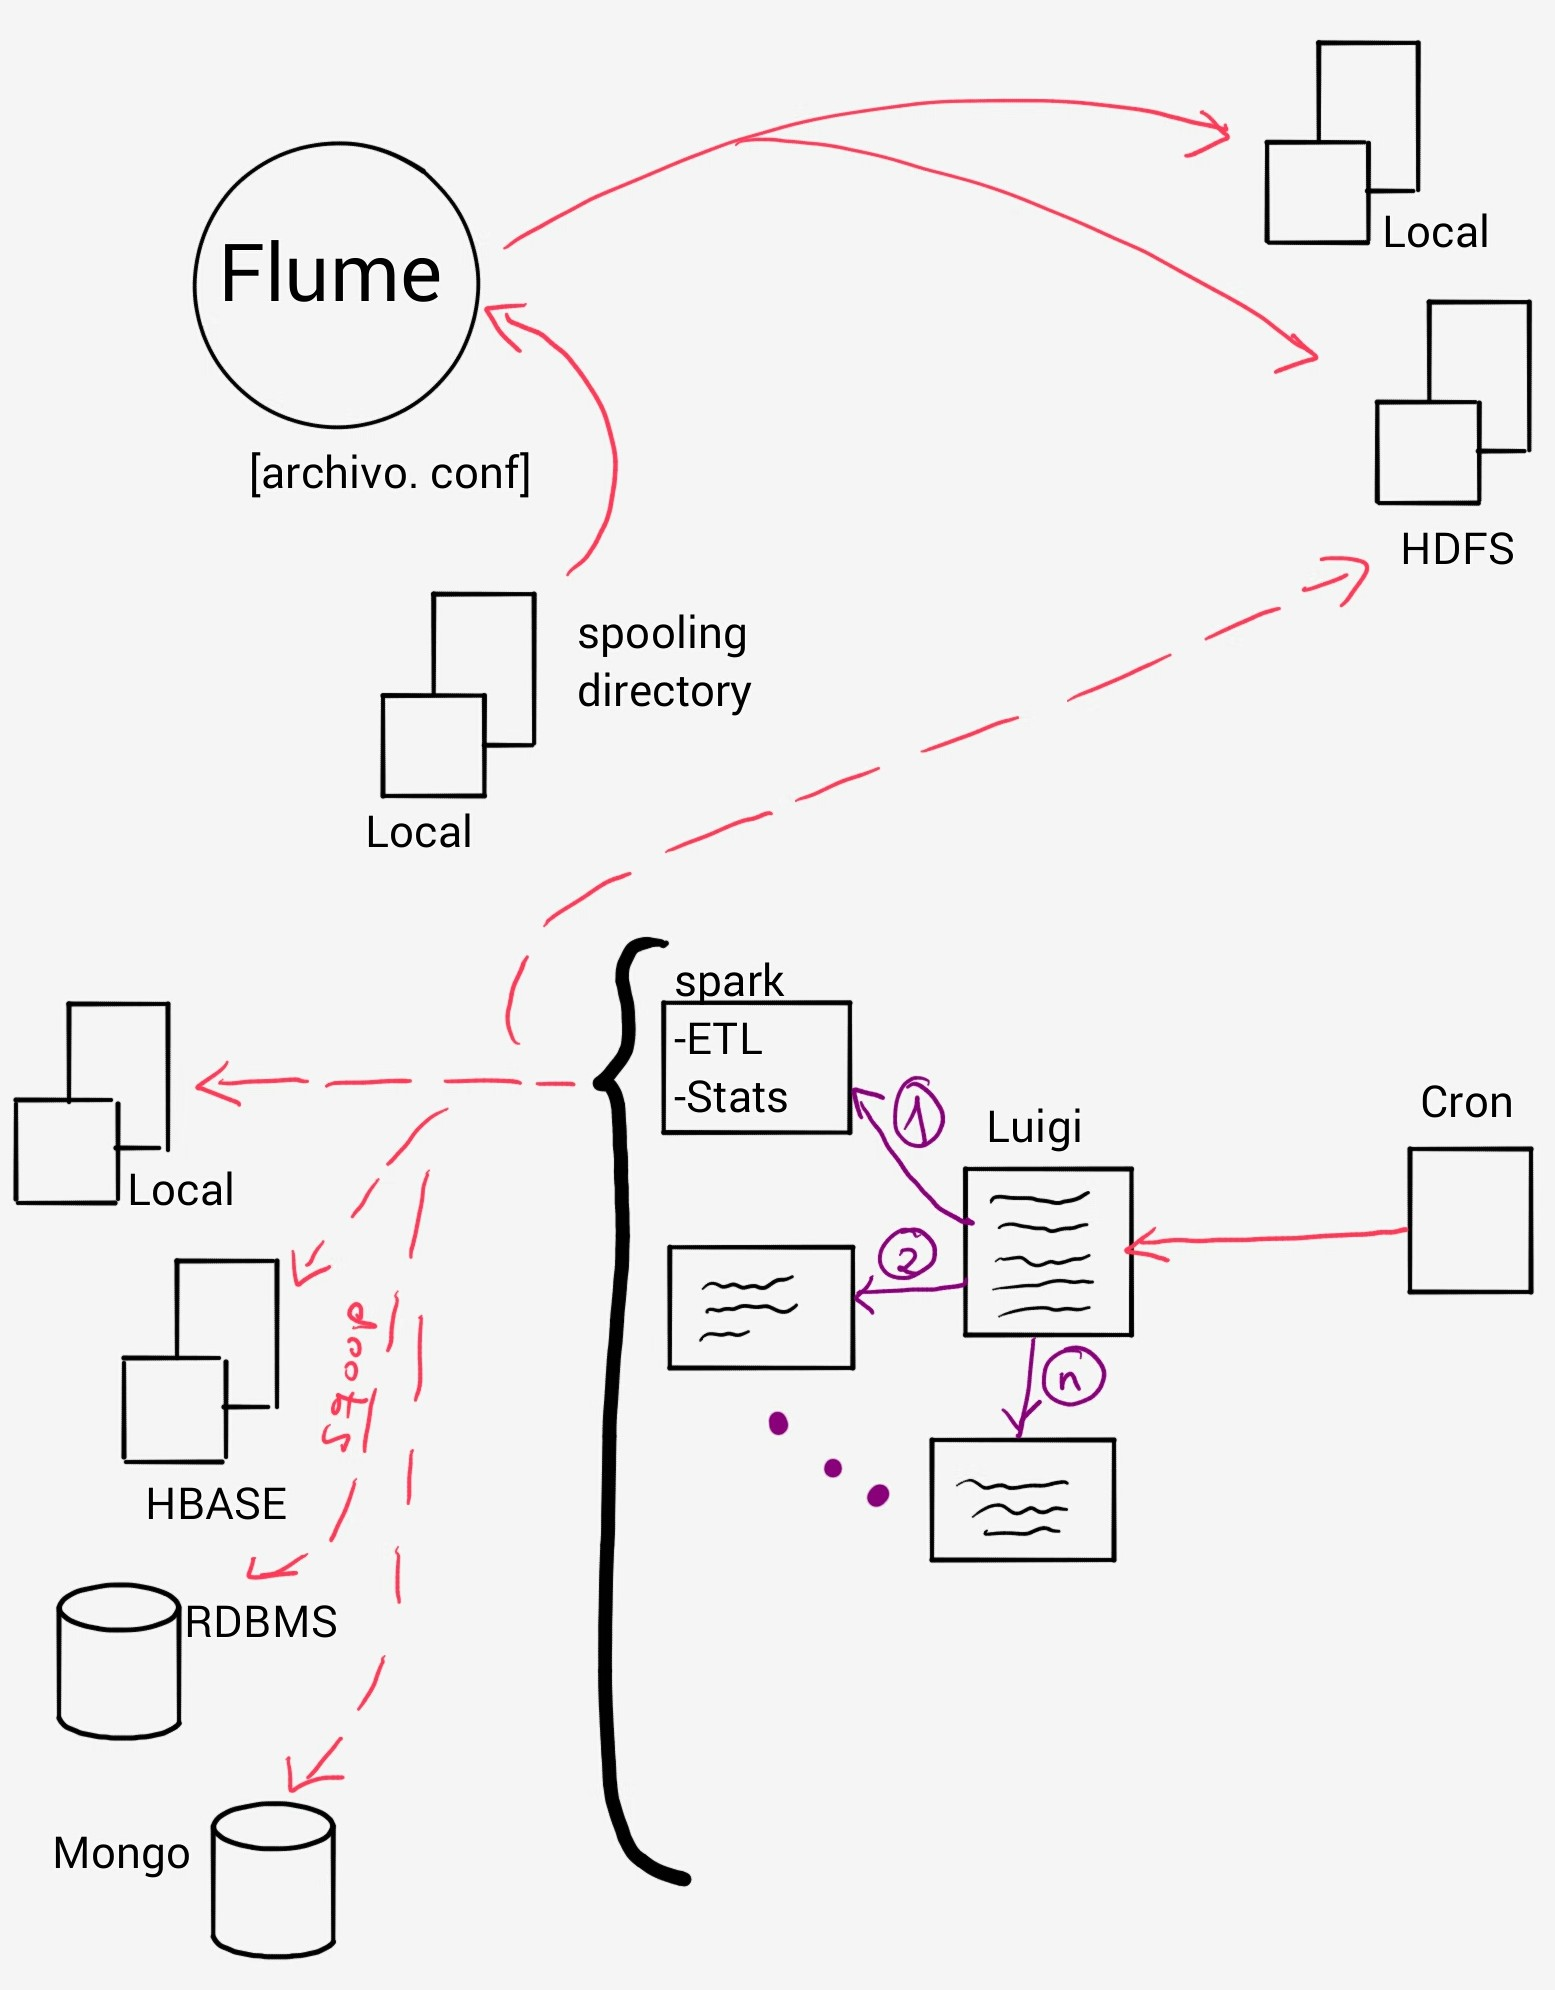
\includegraphics[width=0.8 \textwidth]{img/arquitectura.jpg}
\caption{Flujo de datos implementado.}
\end{figure}

\section{Configuración}\label{configuracion}

\subsection{Docker}\label{docker}

Se utiliza el docker de clase disponible en
\url{https://registry.hub.docker.com/u/nanounanue/docker-hadoop/}. Una
vez bajada la imagen, se levanta el contenedor:

\begin{verbatim}
## Para correr el docker
# Levantamos el contenedor
sudo docker run -ti --name hadoop-pseudo \
    -v /home/animalito/Documents/hadoop_data:/home/itam/data \
    -p 2122:2122 -p 2181:2181 -p 39534:39534 -p 9000:9000 \
    -p 50070:50070 -p 50010:50010 -p 50020:50020 -p 50075:50075 \
    -p 50090:50090 -p 8030:8030 -p 8031:8031 -p 8032:8032 \
    -p 8033:8033 -p 8088:8088 -p 8040:8040 -p 8042:8042 \
    -p 13562:13562 -p 47784:47784 -p 10020:10020 -p 19888:19888 \
    -p 8000:8000 -p 9999:9999 \
    nanounanue/docker-hadoop

# Start: prende el contenedor
# Exec: te conecta al contenedor
sudo docker exec -it hadoop-pseudo /bin/zsh
\end{verbatim}

Después de la ejecución del contenedor, se utiliza el usuario
\texttt{itam} con contraseña \texttt{itam}.

\subsubsection{Permisos}\label{permisos}

Es muy importante dar los permisos apropiados a las carpetas. En el
usuario \texttt{itam} en docker ejecutamos:

\begin{verbatim}
### En el docker, preparamos para el flume
# Permisos para crear carpetitas, en itam
hadoop fs -chown itam /user/itam/datasets/gdelt
chmod -R 777 /opt
sudo chown -R itam /opt/gdelt
\end{verbatim}

\subsection{Carpetas de configuración}\label{carpetas-de-configuracion}

Para que todo funcione, primero se debe configurar una estructura de
carpetas. Se corre entonces, en el docker, con usuario \texttt{itam} el
script de bash \texttt{command\_preparation\_folders.sh}.

\begin{verbatim}
## En local (docker): borro todo
rm -R /home/itam/data/datasets/gdelt/flume_spooldir/*

rm -R /opt/gdelt/log/formato_avro/checkpoint/*
rm -R /opt/gdelt/log/formato_avro/data/*


rm -R /opt/gdelt/log/formato_normal/checkpoint/*
rm -R /opt/gdelt/log/formato_normal/data/*

rm -R /opt/gdelt/log/formato_normal_temp/checkpoint/*
rm -R /opt/gdelt/log/formato_normal_temp/data/*

## En local (docker): creo todos los directorios
mkdir -p /home/itam/data/datasets/gdelt/flume_spooldir
mkdir -p /opt/gdelt/log/formato_normal/checkpoint/
mkdir -p /opt/gdelt/log/formato_normal/data
mkdir -p /opt/gdelt/log/formato_normal_temp/checkpoint/
mkdir -p /opt/gdelt/log/formato_normal_temp/data
mkdir -p /opt/gdelt/log/formato_avro/checkpoint/
mkdir -p /opt/gdelt/log/formato_avro/data


## En el hadoop: borro todos los directorios
hadoop fs -rm -R /user/itam/datasets/gdelt/normal
hadoop fs -rm -R /user/itam/datasets/gdelt/avro
hadoop fs -rm -R /user/itam/datasets/gdelt/temp
hadoop fs -rm -R /user/itam/datasets/gdelt/resultados

## En el hadoop: creo todos los directorios
hadoop fs -mkdir -p /user/itam/datasets/gdelt/normal
hadoop fs -mkdir -p /user/itam/datasets/gdelt/avro
hadoop fs -mkdir -p /user/itam/datasets/gdelt/temp
hadoop fs -mkdir -p /user/itam/datasets/gdelt/resultados


## Para ver donde estan, busco la ruta en el docker para los primeros
## hadoop fs -ls directorio para ver que esta todo en el hadoop
\end{verbatim}

\section{Apache Flume}\label{apache-flume}

\begin{figure}[H]
\centering

\includegraphics[width=0.4 \textwidth]{img/flume1.png}
\end{figure}

\subsection{¿Qué es?}\label{que-es}

\texttt{Flume} es un sistema distribuido y seguro para recoger, agregar
y mover grandes volúmenes de datos provenientes de logs desde distintas
fuentes a un almacén de datos centralizado. La arquitectura de
\texttt{Flume} se puede dividir en seis partes: - Fuente externa. Se
trata de la aplicación o mecanismo, como un servidor web o una consola
de comandos desde la cual se generan eventos de datos que van a ser
recogidos por la fuente. - Fuente. Una fuente es un componente que se
encarga de recoger eventos desde la fuente externa y pasárselos
transaccionalmente al canal. - Canal. Un canal es otro componente que
actuará de almacén intermedio entre la fuente y el sumidero. La fuente
será la encargada de escribir los datos en el canal y permanecerán en él
hasta que el sumidero u otro canal los consuman. - Sumidero. Este
componente será el encargado de recoger los datos desde el canal
intermedio dentro de una transacción y de moverlos a un repositorio
externo. - Repositorio externo. Nos sirve para almacenar en un sistema
de ficheros como puede ser HDFS. - Interceptores. Serán una parte
transversal de la arquitectura y podrán ser relacionados cuando ocurran
distintos tipos de eventos en el flujo. Los interceptores podrán
procesar los datos y añadirles la lógica que se necesite.

\begin{figure}[H]
\centering
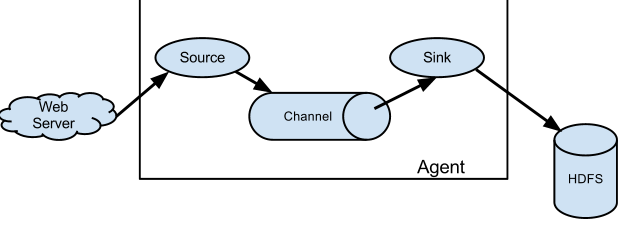
\includegraphics[width=0.8 \textwidth]{img/flume2.png}
\end{figure}

\subsection{¿Para qué se utiliza?}\label{para-que-se-utiliza}

El uso de \texttt{Flume} no sólo se limita a la agregación de datos
desde logs. Debido a que las fuentes de datos son configurables,
\texttt{Flume} permite ser usado para recoger datos desde eventos
ligados al tráfico de red, redes sociales, mensajes de correo
electrónico a casi cualquier tipo de fuente de datos posibles. Flume
soporta cuatro tipos de protocolos para leer datos:

\begin{itemize}
\itemsep1pt\parskip0pt\parsep0pt
\item
  Avro
\item
  Thrift
\item
  Syslog
\item
  Netcat
\end{itemize}

Los distintos componentes de un flujo de eventos en Flume deberán
implementar algún tipo de cliente o servidor que sea compatible con
alguno de los cuatro protocolos anteriores.

Al tratarse de una arquitectura modular podemos concatenar distintos
flujos para hacer un sistema más complejo como puede verse en la
siguiente imagen:

\begin{figure}[H]
\centering
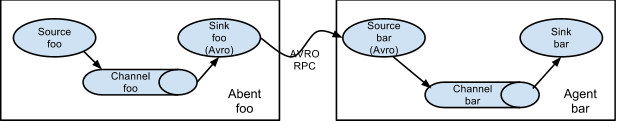
\includegraphics[width=0.8 \textwidth]{img/flume3.png}
\end{figure}

\subsection{Ventajas y desventajas}\label{ventajas-y-desventajas}

Sus principales ventajas:

\begin{itemize}
\itemsep1pt\parskip0pt\parsep0pt
\item
  Permite mover, de manera agregada y eficiente, grandes cantidades de
  datos de resgistro de muchas fuentes diferentes a Hadoop.
\item
  Permite usar como entrada de datos un gran número de fuentes de
  eventos.
\item
  Flume está pensado para procesos en streaming (intentando llegar a
  algo cercano a Real-time).
\item
  Permite definir el flujo de ejecución de manera que podemos indicar
  los componentes por los que va pasando nuestra ejecución. Sus
  principales desventajas:
\item
  cada nodo puede engrentar algunos problemas de rendimiento cuando la
  capacidad de procesamiento de datos del nodo se excede de forma
  inesperada debido a la enorme cantidad de carga de trabajo.
\item
  Si la cantidad de datos transmitidos al nodo es demasiado pequño en
  comparación con su capacidad de procedamiento de datos, el nodo puede
  llegar a ser subtutilizado.`
\end{itemize}

\subsection{Implementación}\label{implementacion-1}

\begin{figure}[H]
\centering
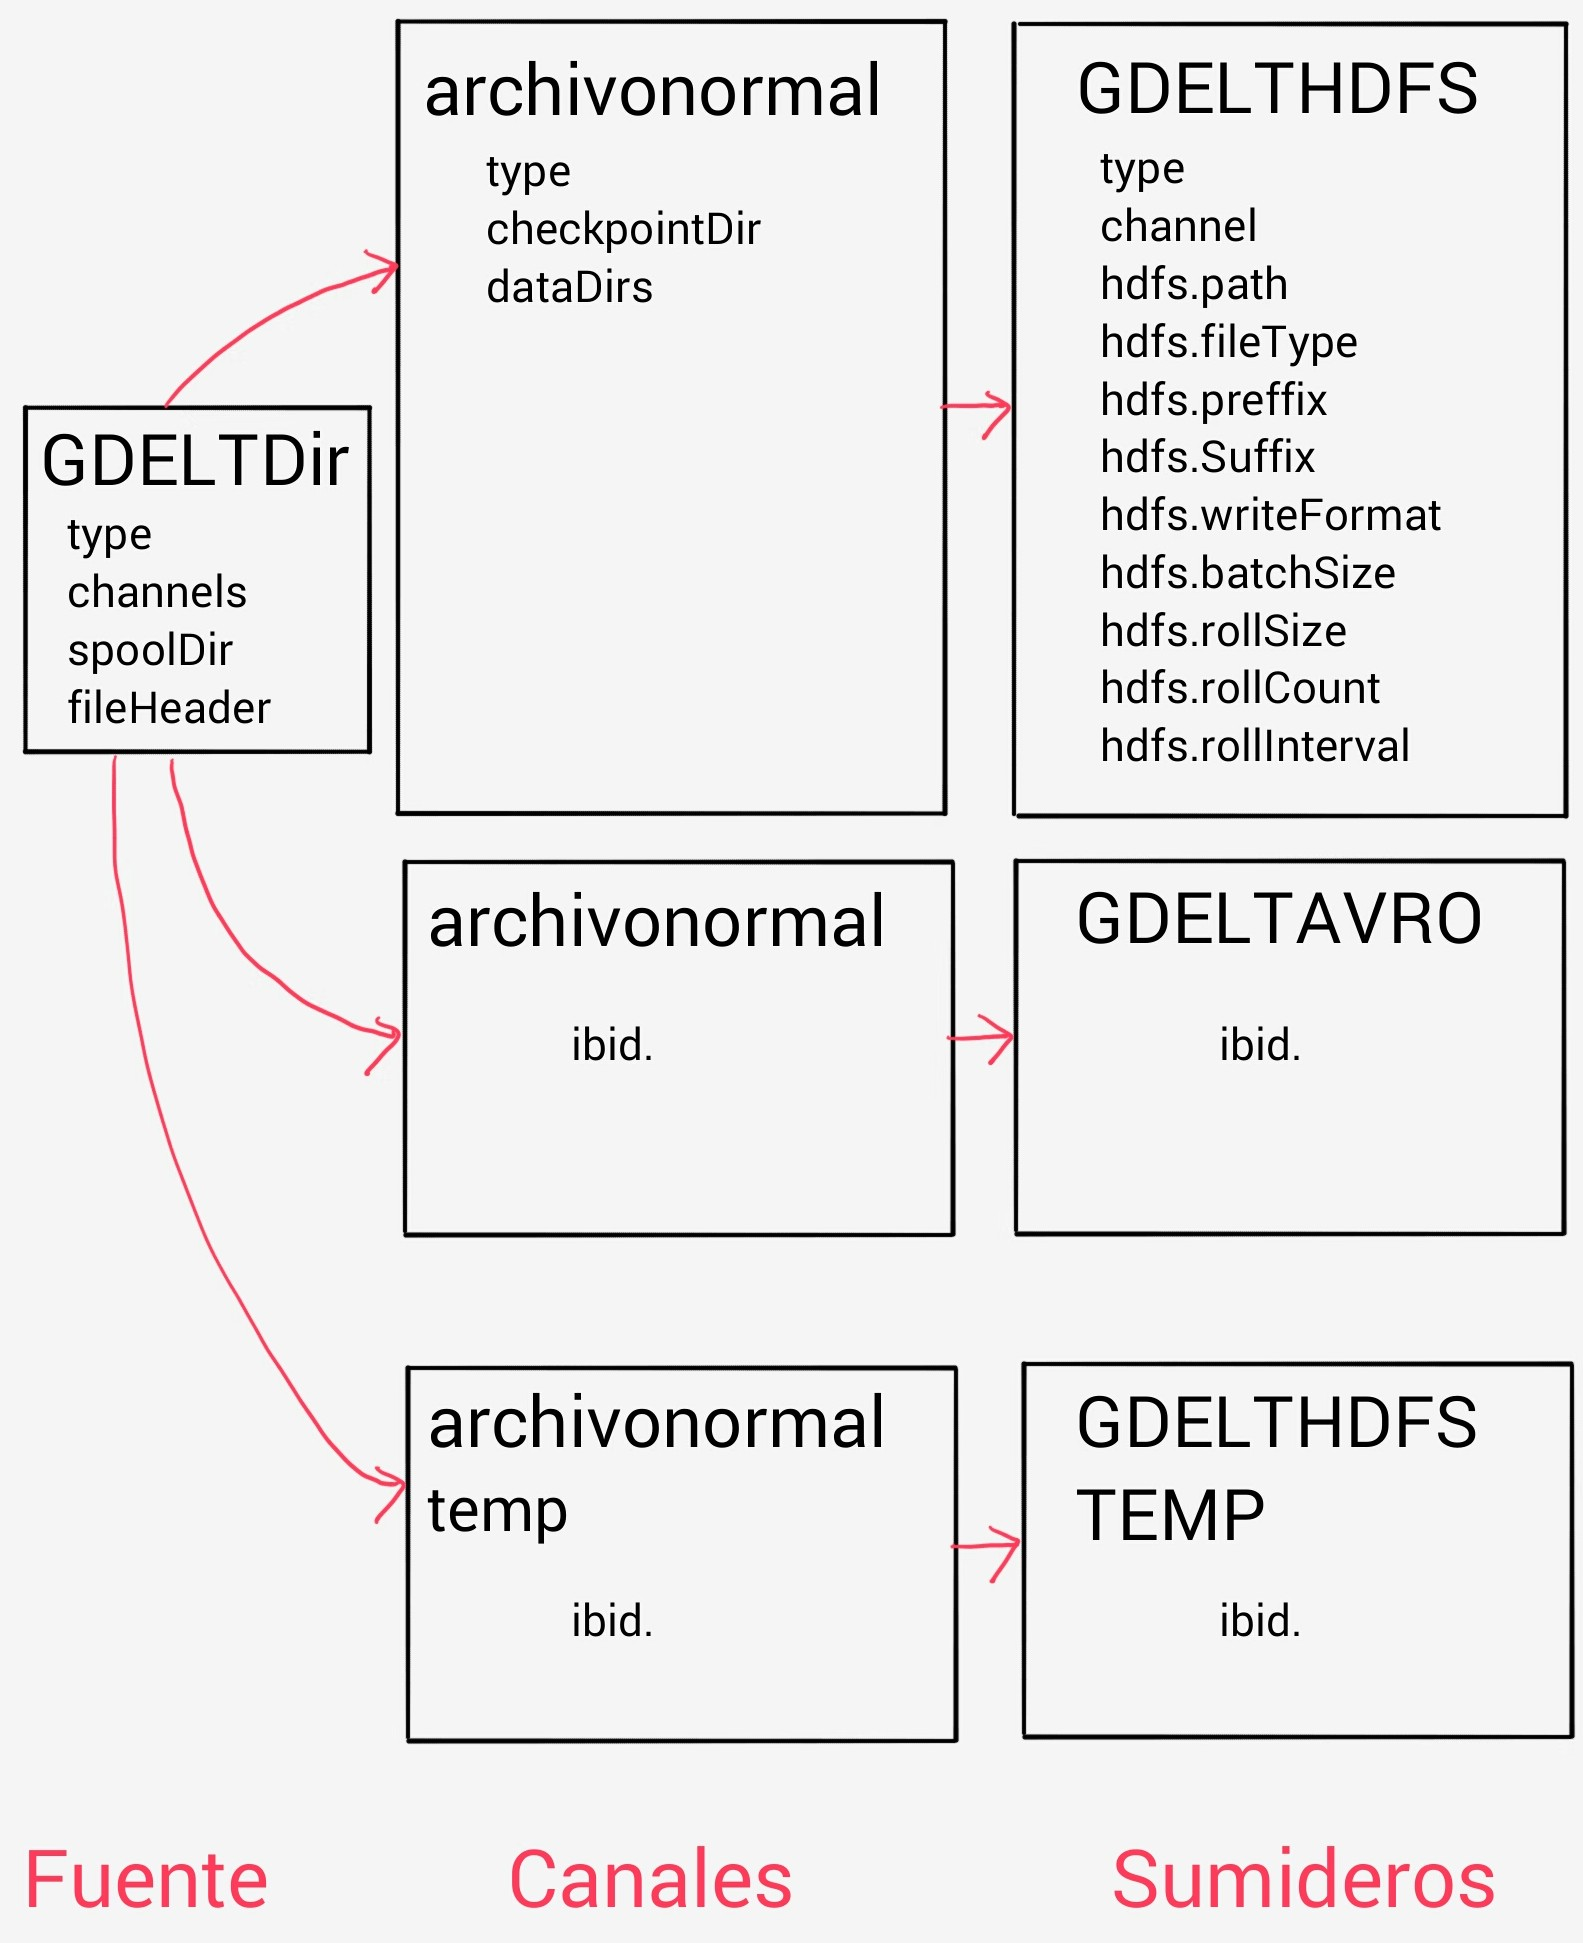
\includegraphics[width=0.8 \textwidth]{img/flume.jpg}
\caption{Fuente, canales y sumideros definidos en \emph{gdelt\_flume\_agent.conf}.}
\label{flume}
\end{figure}

\subsubsection{Configuración}\label{configuracion-1}

Como se muestra en la figura \ref{flume}, la configuración del agente de
flume \texttt{gdelt} necesita que se especifiquen fuente, canales y
sumideros. Asimismo, es necesario que, para cada uno, se definan
mínimamente los atributos en el diagrama. Existen muchos atributos
adicionales que pueden consultarse en
\href{https://flume.apache.org/FlumeUserGuide.html}{la documentación}.

El archivo de configuración utlizado en este ejemplo, se encuentra en
\texttt{conf\_files\textbackslash{}/gdelt\textbackslash{}\_flume\textbackslash{}\_agent.conf}
y se ve como sigue:

\begin{verbatim}
## Los definimos: cuales son (fuente, canales, sumideros)
GDELTAgent.sources = GDELTDir
GDELTAgent.channels = archivonormal archivoavro archivonormaltemp
GDELTAgent.sinks = GDELTHDFS GDELTAVRO GDELTHDFSTEMP

# Fuente e Interceptores
GDELTAgent.sources.GDELTDir.type = spooldir
GDELTAgent.sources.GDELTDir.channels = archivonormal archivoavro archivonormaltemp
GDELTAgent.sources.GDELTDir.spoolDir = /home/itam/data/datasets/gdelt/flume_spooldir
GDELTAgent.sources.GDELTDir.fileHeader = true

# Canales
GDELTAgent.channels.archivonormal.type = file
GDELTAgent.channels.archivonormal.checkpointDir = /opt/gdelt/log/formato_normal/checkpoint/
GDELTAgent.channels.archivonormal.dataDirs = /opt/gdelt/log/formato_normal/data/

GDELTAgent.channels.archivoavro.type = file
GDELTAgent.channels.archivoavro.checkpointDir = /opt/gdelt/log/formato_avro/checkpoint/
GDELTAgent.channels.archivoavro.dataDirs = /opt/gdelt/log/formato_avro/data/

GDELTAgent.channels.archivonormaltemp.type = file
GDELTAgent.channels.archivonormaltemp.checkpointDir = /opt/gdelt/log/formato_normal_temp/checkpoint/
GDELTAgent.channels.archivonormaltemp.dataDirs = /opt/gdelt/log/formato_normal_temp/data/

# Sumideros
GDELTAgent.sinks.GDELTHDFSTEMP.type=hdfs
GDELTAgent.sinks.GDELTHDFSTEMP.channel=archivonormaltemp
GDELTAgent.sinks.GDELTHDFSTEMP.hdfs.path = /user/itam/datasets/gdelt/temp
GDELTAgent.sinks.GDELTHDFSTEMP.hdfs.fileType = DataStream
GDELTAgent.sinks.GDELTHDFSTEMP.hdfs.filePrefix = GDELT-Normal-Data
GDELTAgent.sinks.GDELTHDFSTEMP.hdfs.fileSuffix = .temp
GDELTAgent.sinks.GDELTHDFSTEMP.hdfs.writeFormat = Text
GDELTAgent.sinks.GDELTHDFSTEMP.hdfs.batchSize = 10000
GDELTAgent.sinks.GDELTHDFSTEMP.hdfs.rollSize =  0       
GDELTAgent.sinks.GDELTHDFSTEMP.hdfs.rollCount = 20000000
GDELTAgent.sinks.GDELTHDFSTEMP.hdfs.rollInterval = 180 

GDELTAgent.sinks.GDELTHDFS.type=hdfs
GDELTAgent.sinks.GDELTHDFS.channel=archivonormal
GDELTAgent.sinks.GDELTHDFS.hdfs.path = /user/itam/datasets/gdelt/normal
GDELTAgent.sinks.GDELTHDFS.hdfs.fileType = DataStream
GDELTAgent.sinks.GDELTHDFS.hdfs.filePrefix = GDELT-Normal-Data
GDELTAgent.sinks.GDELTHDFS.hdfs.writeFormat = Text
GDELTAgent.sinks.GDELTHDFS.hdfs.batchSize = 10000
GDELTAgent.sinks.GDELTHDFS.hdfs.rollSize =  0       
GDELTAgent.sinks.GDELTHDFS.hdfs.rollCount = 20000000
GDELTAgent.sinks.GDELTHDFS.hdfs.rollInterval = 180 

GDELTAgent.sinks.GDELTAVRO.type=hdfs
GDELTAgent.sinks.GDELTAVRO.channel=archivoavro
GDELTAgent.sinks.GDELTAVRO.hdfs.path = /user/itam/datasets/gdelt/avro
GDELTAgent.sinks.GDELTAVRO.hdfs.fileType = DataStream
GDELTAgent.sinks.GDELTAVRO.hdfs.filePrefix = GDELT-Avro-Data
GDELTAgent.sinks.GDELTAVRO.hdfs.fileSuffix = .avro
GDELTAgent.sinks.GDELTAVRO.serializer = avro_event
GDELTAgent.sinks.GDELTAVRO.hdfs.batchSize = 10000
GDELTAgent.sinks.GDELTAVRO.hdfs.rollSize  = 0
GDELTAgent.sinks.GDELTAVRO.hdfs.rollCount = 20000000
GDELTAgent.sinks.GDELTAVRO.hdfs.rollInterval = 180 
\end{verbatim}

\subsubsection{Ejecución}\label{ejecucion}

Estos archivos deben estar montados en una carpeta en local para el
docker. De esta manera, con el usuario \texttt{itam}, ejecutamos el
agente de flume de la siguiente manera:

\begin{verbatim}
### Para correr el flume:
## Paso 1
## Corremos flume desde docker, su itam
flume-ng agent -n GDELTAgent --conf ingestion -f /home/itam/data/conf_files/gdelt_flume_agent.conf
## Paso 2
## Copias el archivo que quieres trepar a la carpeta `flume_spooldir`
\end{verbatim}

Con el agente de flume prendido, solo es necesario copiar los archivos
en el \texttt{spoolDir} definido en la configuraciön para que el agente
los procese e inserte en el HDFS y avro.

Si todo esta apropiadamente configurado, entonces al copiar un archivo
de \texttt{gdelt} en el \texttt{spoolDir} local (sobre el cual se monta
el \texttt{docker}) inmediatamente se activan los procesos del agente
gdelt.

\begin{figure}[H]
\centering
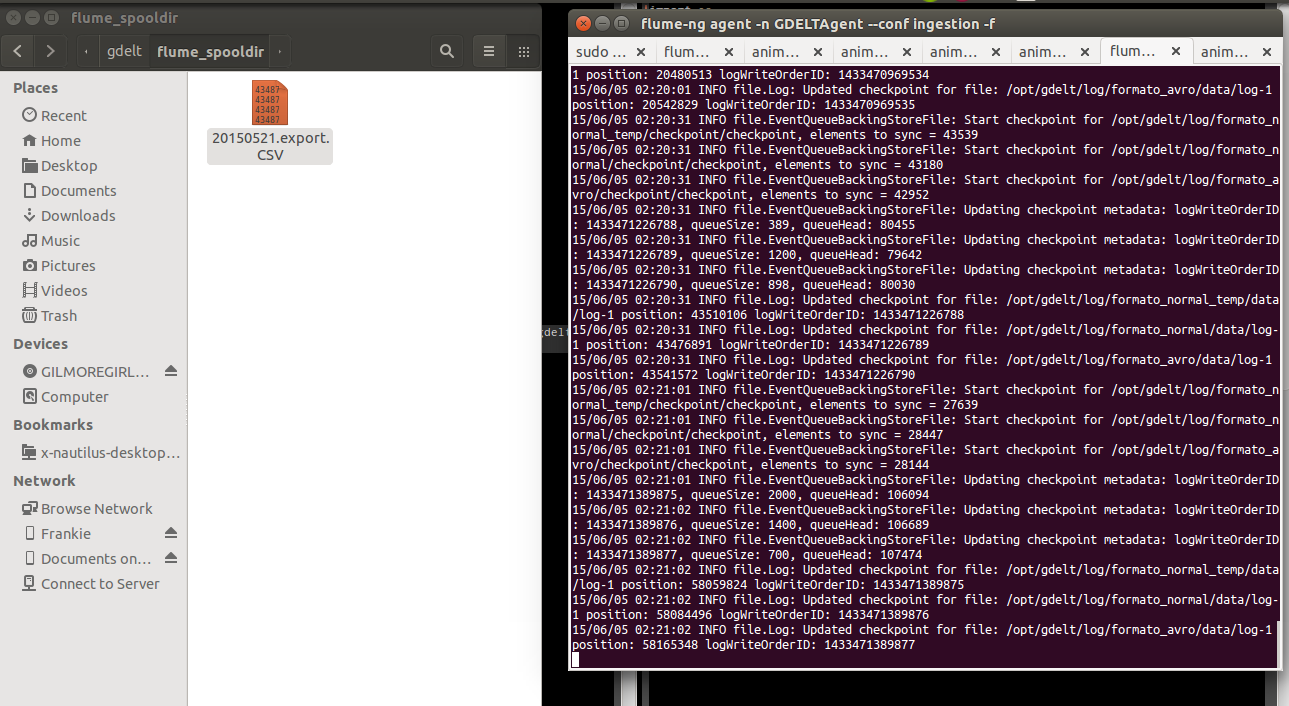
\includegraphics[width=0.9\textwidth]{img/ejecucion_flume.png}
\end{figure}

\section{Spark}\label{spark}

\begin{figure}[H]
\centering

\includegraphics[width=0.4 \textwidth]{img/spark1.png}
\end{figure}

\subsection{¿Qué es?}\label{que-es-1}

\texttt{Spark} es una plataforma de computación de código abierto para
análisis y procesos avanzados. Desde su principio \texttt{Spark} fue
diseñado para soportar en memoria algoritmos iterativos que se pudieran
desarrollar sin escribir un conjunto de resultados cada vez que
procesaba un dato. Esta habilidad para mantener todo en memoria es una
técnica de computación de alto rendimiento aplicado al análisis
avanzado.

\subsection{¿Para qué se utiliza?}\label{para-que-se-utiliza-1}

\texttt{Spark} es utilizado para implementar análisis avanzados, cuenta
con un \texttt{framework} que incluye:

\begin{itemize}
\itemsep1pt\parskip0pt\parsep0pt
\item
  La librería Mlib para implementar funciones para Machine Learning.
\item
  El motor de gráficos GraphX.
\item
  \texttt{Spark Streaming} para procesar en tiempo real grandes
  cantidades de datos.
\item
  \texttt{Sparck SQL} para procesar consultas en \texttt{SQL}.
\end{itemize}

\begin{figure}[H]
\centering
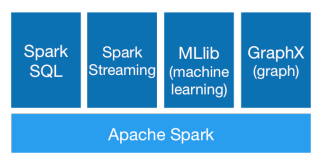
\includegraphics[width=0.8 \textwidth]{img/spark2.png}
\end{figure}

Esta plataforma asegura a los usuarios la consistencia en los resultados
a través de distintos tipos de análisis.

\subsection{Ventajas y desventajas}\label{ventajas-y-desventajas-1}

Sus principales ventajas:

\begin{itemize}
\itemsep1pt\parskip0pt\parsep0pt
\item
  Capacidad de procesamiento en memoria, \texttt{Spark} tiene
  velocidades de procesamiento hasta 100 veces más rápidas que las
  conseguidas utilizando \texttt{MapReduce}.
\item
  Esquema de computación más flexible que \texttt{MapReduce}.
\item
  Se puede descargar y ejecutar desde un ordenador personal.
\item
  Actualmente \texttt{Spark} es apoyado comercialmente por
  \texttt{Cloudera}, \texttt{Hortonworks} y \texttt{DataBricks}.
\item
  Se pueden desarrollar aplicaciones en \texttt{Spark} utilizando
  \texttt{Java}, \texttt{Scala}, \texttt{Phyton} y \texttt{R}.
\item
  Unificación del streaming en tiempo real.
\end{itemize}

\begin{figure}[H]
\centering
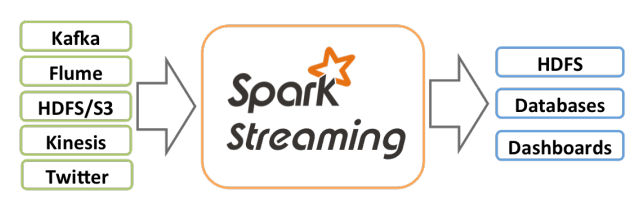
\includegraphics[width=0.8 \textwidth]{img/spark3.png}
\end{figure}

\begin{itemize}
\itemsep1pt\parskip0pt\parsep0pt
\item
  Permite integrarse con una gran cantidad de fuentes y repositorios de
  datos.
\end{itemize}

\begin{figure}[H]
\centering
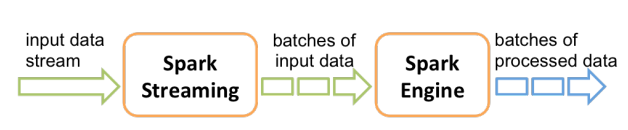
\includegraphics[width=0.8 \textwidth]{img/spark4.png}
\end{figure}

Sus principales desventajas:

\begin{itemize}
\itemsep1pt\parskip0pt\parsep0pt
\item
  Consume mucha memoria
\item
  Solo soporta los sistemas de archivo a través de \texttt{HDFS}
\end{itemize}

\subsection{Implementación}\label{implementacion-2}

En el archivo \texttt{workflows/pyspark\_script.py} se especifican las
tareas de limpieza que debe realizar el spark y que, después, serán
ejecutadas por el orquestador.

\begin{verbatim}
import os
import csv
from io import StringIO
import sys
from pyspark import SparkContext, SparkConf


def load_tsv(archivo):
    return csv.reader(StringIO(archivo[1]), delimiter="\t")

def limpia_informacion(line): 
    
    return  [line[0], line[1], line[3], line[2].replace(line[3],""),line[1].replace(line[2],"")] + \
        line[5:]

def main_limpia_info(args):
    try:
        conf = (SparkConf().setMaster("local").setAppName("GdeltImportingInfo"))
        sc = SparkContext(conf = conf)  
        obs = sc.textFile("hdfs://localhost/user/itam/datasets/gdelt/temp/*.temp").\
            map(lambda x: x.split("\t") ).map(limpia_informacion)

        obs_mexico = obs.filter(lambda line: line[5] == "MEX" or line[15] == "MEX").map(lambda x: "\t".join(x))
        obs = obs.map(lambda x: "\t".join(x))
        obs_mexico.saveAsTextFile("hdfs://localhost/user/itam/datasets/gdelt/resultados/mexico")
        obs.saveAsTextFile("hdfs://localhost/user/itam/datasets/gdelt/resultados/general")
        #print obs_mexico.take(5)
        print "Ejecucion exitosa de limpieza\n"
    except: 
        print "Ejecucion fallida de limpieza\n"

if __name__ == '__main__':
    #print "Ejecucion de PySpark"
    if sys.argv[1] == "limpieza_datos":
        main_limpia_info(sys.argv)
    #print "Fin de ejecucion"
\end{verbatim}

\section{Sqoop}\label{sqoop}

\begin{figure}[H]
\centering

\includegraphics[width=0.8 \textwidth]{img/sqoop1.png}
\end{figure}

\subsection{¿Qué es?}\label{que-es-2}

\texttt{Sqoop} es una librería que permite importar datos desde un
almacenamiento de datos estructurado, como una base de datos relacional,
a \texttt{Hadoop}. \texttt{Sqoop} también permite importar datos a otras
bases de datos como \texttt{Hive} o \texttt{HBase}.

\subsection{¿Para qué se utiliza?}\label{para-que-se-utiliza-2}

\texttt{Sqoop} suministra una herramienta desde línea de comando a
través de la cual se puede realizar todo el proceso de importación y
exportación de datos desde una base de datos relacional a un sistema de
ficheros distribuidos y viceversa.

\subsection{Ventajas y desventajas}\label{ventajas-y-desventajas-2}

Sus principales ventajas:

\begin{itemize}
\itemsep1pt\parskip0pt\parsep0pt
\item
  Agiliza y facilita el movimiento de datos dentro y fuera de Hadoop.
\item
  Sqoop está enfocado a bases de datos relacionales.
\item
  Sqoop utiliza durante su ejecucción el paradigma MapReduce. Lo que
  permite procesar la información de manera paralela en procesos batch.
\item
  Lanza directamente una o varias tareas MapReduce para procesar los
  datos.
\end{itemize}

Sus principales desventajas:

\begin{itemize}
\itemsep1pt\parskip0pt\parsep0pt
\item
  Solamente realiza la validación a los datos copiados de una sola tabla
  en \texttt{HDFS}.
\end{itemize}

\subsection{Implementación}\label{implementacion-3}

En este caso, no se llamó a sqoop en el orquestador. Sin embargo, se
extrae la base de datos a \texttt{hive} directo y se crean las tablas
para realizar los queries. Los archivos de hive pueden ser llamados por
el orquestador de manera directa y que el flujo esté completo.

Los ejemplos de hive y los scripts de creación de las tablas tomandolas
del HDFS son \texttt{load\_etled.q} para la base que ya pasó por el
orquestador. Además, se puede cargar de manera directa la base normal o
temporal del HDFS con \texttt{load\_original.q}. El primero, se ve como
sigue:

\begin{verbatim}
create table gdeltetled
(GLOBALEVENTID BIGINT, 
SQLDATE INT, 
Year INT, 
Month INT, 
Day INT,
FractionDate DECIMAL, 
Actor1Code STRING, 
Actor1Name STRING, 
Actor1CountryCode STRING, 
Actor1KnownGroupCode STRING, 
Actor1EthnicCode STRING, 
Actor1Religion1Code STRING, 
Actor1Religion2Code STRING, 
Actor1Type1Code STRING, 
Actor1Type2Code STRING, 
Actor1Type3Code STRING, 
Actor2Code STRING, 
Actor2Name STRING, 
Actor2CountryCode STRING, 
Actor2KnownGroupCode STRING, 
Actor2EthnicCode STRING, 
Actor2Religion1Code STRING, 
Actor2Religion2Code STRING, 
Actor2Type1Code STRING, 
Actor2Type2Code STRING, 
Actor2Type3Code STRING, 
IsRootEvent BOOLEAN, 
EventCode STRING,
EventBaseCode STRING, 
EventRootCode STRING, 
QuadClass INT, 
GoldsteinScale DECIMAL, 
NumMentions BIGINT, 
NumSources BIGINT, 
NumArticles BIGINT, 
AvgTone DECIMAL, 
Actor1Geo_Type BIGINT, 
Actor1Geo_FullName STRING, 
Actor1Geo_CountryCode STRING, 
Actor1Geo_ADM1Code STRING, 
Actor1Geo_Lat DECIMAL, 
Actor1Geo_Long DECIMAL, 
Actor1Geo_FeatureID DECIMAL, 
Actor2Geo_Type BIGINT, 
Actor2Geo_FullName STRING, 
Actor2Geo_CountryCode STRING, 
Actor2Geo_ADM1Code STRING, 
Actor2Geo_Lat DECIMAL, 
Actor2Geo_Long DECIMAL, 
Actor2Geo_FeatureID DECIMAL, 
ActionGeo_Type BIGINT, 
ActionGeo_FullName STRING, 
ActionGeo_CountryCode STRING, 
ActionGeo_ADM1Code STRING, 
ActionGeo_Lat DECIMAL, 
ActionGeo_Long DECIMAL, 
ActionGeo_FeatureID DECIMAL, 
DATEADDED BIGINT, 
SOURCEURL STRING)
row format delimited fields terminated by '\t' stored as textfile;

LOAD DATA INPATH '/user/itam/datasets/gdelt/resultados/mexico/part-00000' OVERWRITE INTO TABLE gdeltetled;
\end{verbatim}

Ejemplos de los queries de analítica que se pueden realizar son:

\begin{verbatim}
CREATE TABLE actiontypes AS
select gdeltetled.actiongeo_type, count (DISTINCT gdeltetled.globaleventid) from gdeltetled group by gdeltetled.actiongeo_type;
\end{verbatim}

\section{Orquestación vía Luigi}\label{orquestacion-via-luigi}

\begin{figure}[H]
\centering

\includegraphics[width=0.4 \textwidth]{img/luigi.jpeg}
\end{figure}

\subsection{¿Qué es?}\label{que-es-3}

\texttt{Luigi} es una herramienta de generación de \texttt{workflows} y
\texttt{pipelines} de trabajo. Permite definir distintos tipos de
tareas, así como las dependencias de ejecución entre ellas, además de
disponer de una interfaz de visualización para comprobar el estado de la
ejecución y de la finalización del \texttt{workflow} completo. Está
escrito en \texttt{Python}, y tiene plantillas predefinidas para varios
tipos de tareas.

\subsection{¿Para qué se utiliza?}\label{para-que-se-utiliza-3}

Permite gestionar la dependencia entre tareas mediante una serie de
funciones que se deben reescribir. Las más importantes son las
siguiente:

\begin{itemize}
\itemsep1pt\parskip0pt\parsep0pt
\item
  Run. Esta función contendrá el código principal de la tarea que se
  desea ejecutar.
\item
  Requires. La función requires establece la relación de dependencia
  entre dos tareas.
\item
  Output. La función output especifica la referencia al contenido que la
  tarea genera. Si se lanza varias veces el mismo \texttt{workflow},
  antes de ejecutar cada una de las tareas, \texttt{Luigi} comprobará
  que no exista la referencia marcada en el \texttt{output}. En caso de
  que exista, la tarea se marcará como completada y pasará a la
  siguiente.
\end{itemize}

\subsection{Ventajas y desventajas}\label{ventajas-y-desventajas-3}

\subsection{Implementación}\label{implementacion-4}

\begin{figure}[H]
\centering
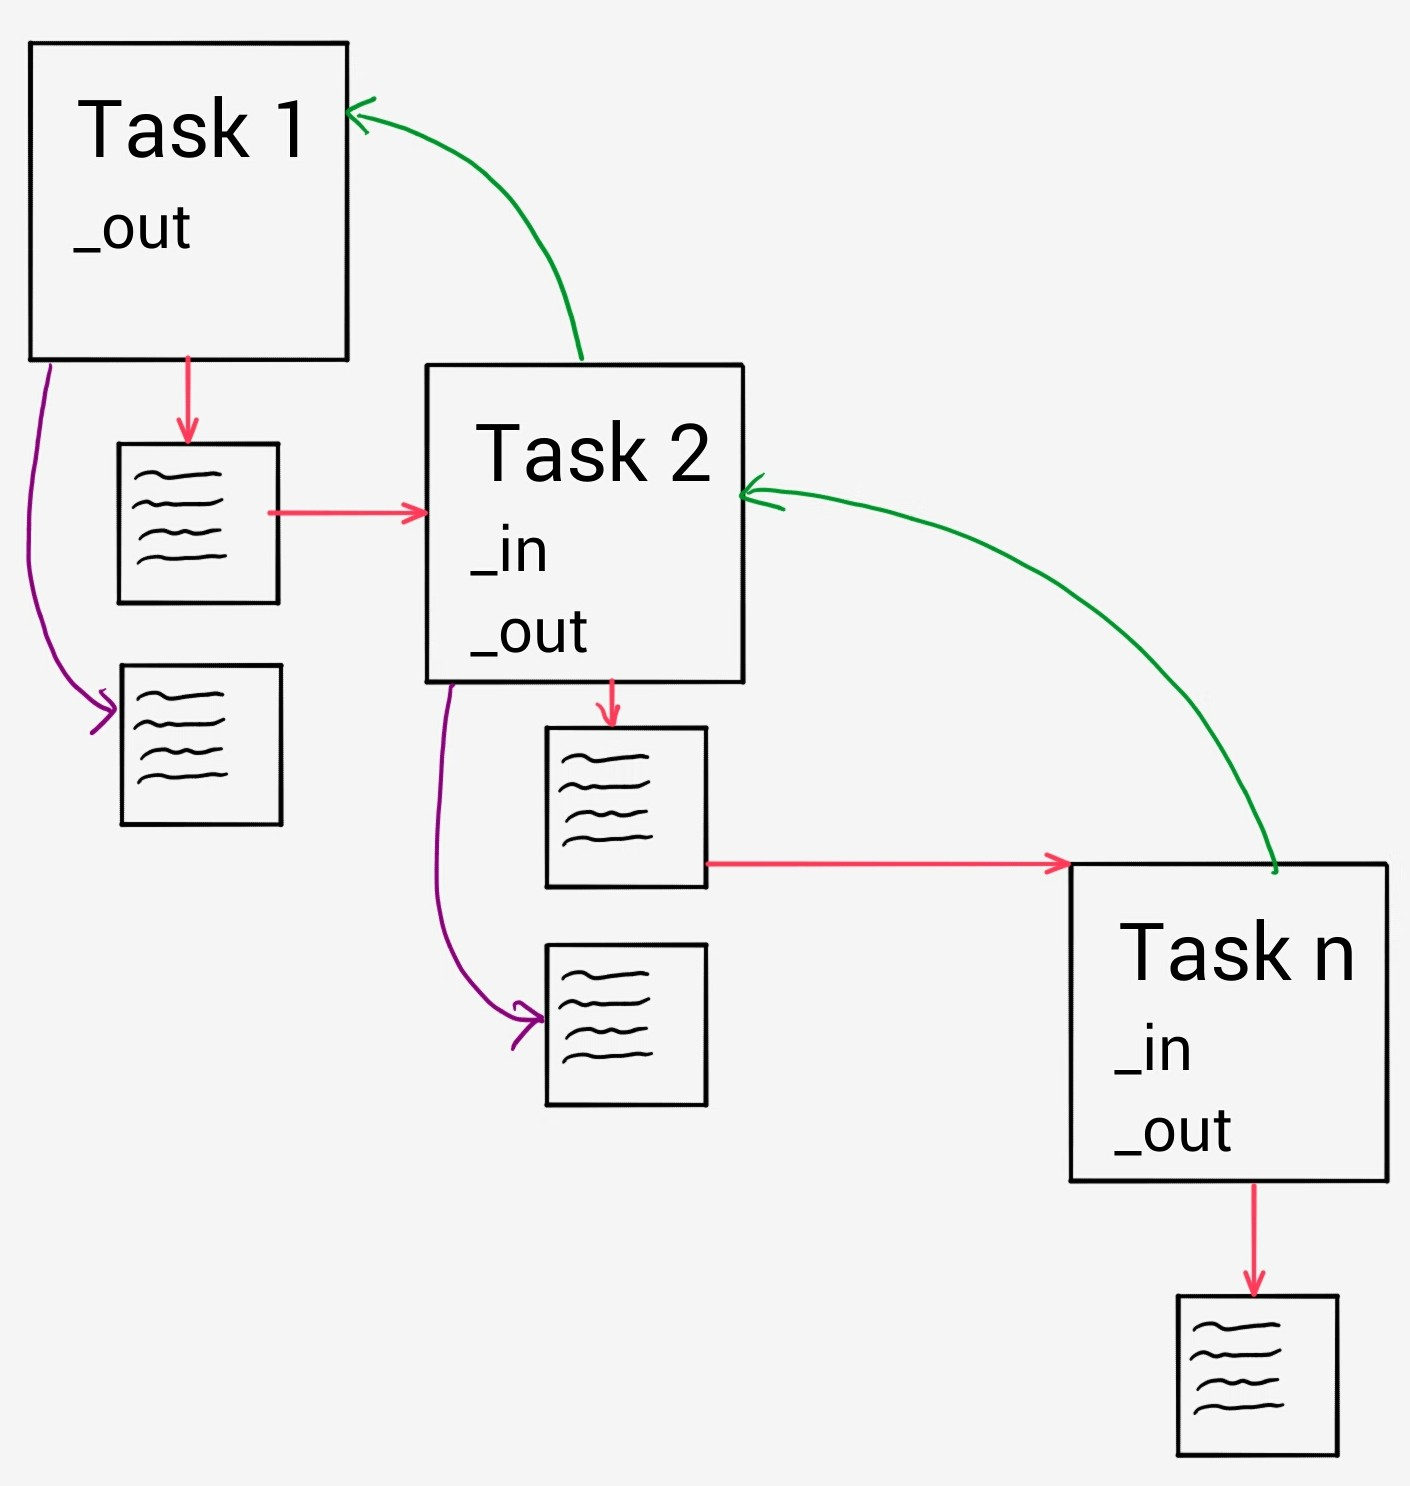
\includegraphics[width=0.8 \textwidth]{img/luigi.jpg}
\caption{Esquema de las tareas implementadas en \emph{orquestador\_gdelt.py}.}
\end{figure}

\section{Hive}\label{hive}

\begin{figure}[H]
\centering

\includegraphics[width=0.3 \textwidth]{img/hive1.png}
\end{figure}

\subsection{¿Qué es?}\label{que-es-4}

\texttt{Hive} es un sistema de almacén de datos que facilita el manejo
sencillo de datos, consultas ad-hoc, y el análisis de grandes conjuntos
de datos almacenados en sistemas de ficheros compatibles con
\texttt{Hadoop}.

Algunas de las principales características de \texttt{Hive} y de su
lenguaje \texttt{HiveQL} son las siguientes:

\begin{itemize}
\itemsep1pt\parskip0pt\parsep0pt
\item
  \texttt{HiveQL} es un lenguaje tipo \texttt{SQL} que permite realizar
  consultas de grandes volúmenes de datos almacenados en un sistema de
  ficheros compatible con \texttt{Hadoop}.
\item
  Las consultas realizadas desde \texttt{HiveQL} se ejecutan siguiendo
  el modelo \texttt{MapReduce}.
\item
  \texttt{Hive} necesita almacenar metadatos y los esquemas de datos
  mediante un servicio metastore.
\item
  El programador no necesita \texttt{HiveQL} ningún maper o reducer lo
  que agiliza el desarrollo. \texttt{Hive} se encarga de traducir la
  consulta escrita con \texttt{HiveQL} en tareas \texttt{MapReduce}.
\item
  \texttt{Hive} permite que el programador pudiera escribir sus propios
  mares y reduces si fuera necesario
\item
  \texttt{HiveQL} no permite inserción, actualización o borrado de datos
  a nivel de registro. Tampoco dota de transaccionalidad a sus
  consultas.
\item
  Permite crear tablas y insertar datos que están almacenados en el
  sistema de ficheros de \texttt{Hadoop}.
\item
  La latencia de las consultas suele ser mayor que las realizadas en las
  bases de datos relacionales debido a la inicialización de
  \texttt{MapReduce}.
\item
  Schema on read vs schema on write. A diferencia de las bases de datos
  relacionales que garantizan que el \texttt{Schema} se cumple cuando se
  inserta un registro, \texttt{Hive} no garantiza esto aunque intenta
  garantizar el esquema en las lecturas.
\end{itemize}

\subsection{¿Para qué se utiliza?}\label{para-que-se-utiliza-4}

Hive provee un mecanismo para dotar de estructura en los datos y
realizar consultas sobre los mismos con el lenguaje tipo SQL llamado
HiveQL. Al mismo tiempo este lenguaje también permite a los
programadores de \texttt{MapReduce} incluir sus propios mappers y
reducers cuando no sea conveniente o eficiente expresar esta lógica con
HiveQL.

\subsection{Ventajas y desventajas}\label{ventajas-y-desventajas-4}

Se recomienda utilizar \texttt{Hive} para el procesamiento secuencial de
grandes archivos de datos multi-estructurados. Las principales ventajas
de \texttt{Hive} son:

\begin{itemize}
\itemsep1pt\parskip0pt\parsep0pt
\item
  Su capacidad de mejorar la simplicidad y la rapidez del desarrollo de
  \texttt{MapReduce}.
\item
  Hace más sencillo el procesamiento de archivos relacionados entre sí.
\item
  Utiliza queries similares a \texttt{SQL}.
\end{itemize}

Las principales desventajas de \texttt{Hive} son:

\begin{itemize}
\itemsep1pt\parskip0pt\parsep0pt
\item
  No está completamente aislado del sistema de archivos subyacente, esto
  implica que con frecuencia el usuario requiere ayuda del optimizador
  con construcciones del lenguaje para procesar consultas más complejas.
\item
  No puede sustituir a la funcionalidad, facilidad de uso, el
  rendimiento y la madurez de un \texttt{DBMS}.
\end{itemize}

\subsection{Implementación}\label{implementacion-5}

Desde python, utilizando luigi, es posible que, después de la ejecución
del agente de flume, los procesos de limpieza, transformación y carga de
datos (a hive, pig o postgres) sean realizados de manera automática.
Cada tarea se ejecuta si (y solo si) la tarea previa fue ejecutada de
manera exitosa. Debido a que la tarea posterior debe leer un archivo
generada por la tarea previa, se decidió que cada tarea regresara por un
lado los flujos de datos y, por otro, un archivo con el log de la tarea
previa. En caso de que ésta es exitosa, entonces se realiza la
siguiente. El código es como sigue:

\begin{verbatim}
import luigi
from luigi.hdfs import HdfsTarget
import os
from io import StringIO
import sys

class LimpiaInformacionTask(luigi.Task):
    
    def output(self):
        return HdfsTarget("/user/itam/datasets/gdelt/resultados/limpieza_info.txt")
    
    def run(self):
        _out = self.output().open("w")
        try: 
            f = os.popen('nohup spark-submit /home/itam/workflows/pyspark_script.py limpieza_datos &')
            res_exec = f.read()
            _out.write("Ejecucion exitosa de LimpiarInformacionTask \n")
            _out.write(str(res_exec) + "\n")
            #print res_exec
        except:
            _out.write("Ejecucion fallida")
        _out.close()

class AnalizaInformacionTask(luigi.Task):

    def requires(self):
        return LimpiaInformacionTask()

    def output(self):
        return HdfsTarget("/user/itam/datasets/gdelt/resultados/analisis_info.txt")

    def run(self):
        #print "\n\n\nInicia ejecucion de analisis de informacion\n\n\n"
        try:
            _in = self.input().open("r")
            _out = self.output().open("w")
            for line in _in:
                _out.write(line) 
                #print line + "\n"
            _in.close()
            _out.close()
        except:
            print "\nERROR  EN ANALISIS DE INFORMACION\n"

class ExportaInformacionTask(luigi.Task):

    def output(self):
        return HdfsTarget("/user/itam/datasets/gdelt/resultados/exportacion_info.txt")

    def requires(self):
        return AnalizaInformacionTask()

    def run(self):
        _in = self.input().open("r")
        _out = self.output().open("w")
        for line in _in:
            _out.write(line)

        _out.close()
        _in.close()


if __name__ == '__main__':
    luigi.run(main_task_cls=ExportaInformacionTask)
\end{verbatim}

Este archivo está en \texttt{workflows/orquestador\_gdelt.py}, se llama
desde el docker con usuario \texttt{itam} y ejecuta también las tareas
especificadas en pyspark.

\section{Conclusiones}\label{conclusiones}

El flujo implementado es muy simple y se realizó de manera local. Sin
embargo, la configuración es fácilmente extendible. Además, las tareas
realizadas a través del orquestador pueden ser tan complicadas como un
necesite.

\end{document}
